\documentclass[xcolor={dvipsnames}]{beamer}
% For more themes, color themes and font themes, see:
% http://deic.uab.es/~iblanes/beamer_gallery/index_by_theme.html
\mode<presentation>
{
	\usetheme{EastLansing}      % or try Darmstadt, Madrid, Warsaw, ...
	% \usecolortheme{rose} % or try albatross, beaver, crane, ...
	\usefonttheme{default}  % or try serif, structurebold, ...
	\setbeamertemplate{navigation symbols}{}
	\setbeamertemplate{caption}[numbered]
	\definecolor{myblue}{RGB}{74,60,137}
	\setbeamercolor*{structure}{bg=myblue!20,fg=myblue}
	
	\setbeamercolor*{palette primary}{use=structure,fg=white,bg=structure.fg}
	\setbeamercolor*{palette secondary}{use=structure,fg=white,bg=structure.fg!75}
	\setbeamercolor*{palette tertiary}{use=structure,fg=white,bg=black}
	\setbeamercolor*{palette quaternary}{fg=white,bg=black}
	
	\setbeamercolor{section in toc}{fg=black,bg=white}
	\setbeamercolor{alerted text}{use=structure,fg=structure.fg!50!black!80!black}
	
	\setbeamercolor{titlelike}{parent=palette primary,fg=structure.fg!50!black}
	\setbeamercolor{frametitle}{bg=myblue!85,fg=white}
	
	\setbeamercolor*{titlelike}{parent=palette primary}
	
} 


\usepackage[english]{babel}
\usepackage[utf8x]{inputenc}
\usepackage{subfig}
\usepackage{listings}
\usepackage{lstautogobble}
\usepackage{multicol}
\usepackage{hyperref}


\title[Local interpretability]{Explaining single prediction}
\author{Mateusz Staniak}
\institute{University of Wroc{\l}aw}
\date{Budapest, 12.05.2017}

\begin{document}
	
\lstset{language=R,
	basicstyle=\ttfamily\scriptsize,
	keywordstyle=\color{blue}\ttfamily,
	stringstyle=\color{red}\ttfamily,
	commentstyle=\color{green}\ttfamily
	autogobble=true
}
	

	\begin{frame}
		\titlepage
	\end{frame}
	
	\section{Introduction}
	
	\begin{frame}{Outline}
		\begin{enumerate}
			\item Intro
			
			\item Predictions breakdown
			
			\begin{itemize}
				\item breakDown package
				
				\item Shapley values
			\end{itemize}

			
			\item Local approximations
			
			\begin{itemize}
				\item LIVE (Local Interpretable Visual Explanations)
				
				\item LIME (Locally Interpretable Model-agnostic Explanations)
			\end{itemize}
			
			\item Summary
			
		\end{enumerate}
	\end{frame}
	
	\begin{frame}{Why explain a single prediction? - bird's-eye view}
		
		
\includegraphics[scale=0.85]{ilustracje_erum/bird.jpg}
		
		\begin{itemize}
			
			\item when important decision are made based on ML model, it needs to be \textbf{trustworthy}
			
			\item trust comes from \textbf{understanding}
			
			\item the demand for interpretable algorithms is growing
			(see: \textit{Weapons of math destruction}, Facebook feed controversies etc.)
		\end{itemize}
	\end{frame}

	
	\begin{frame}{Why explain a single prediction? - worm-eye view}
	
	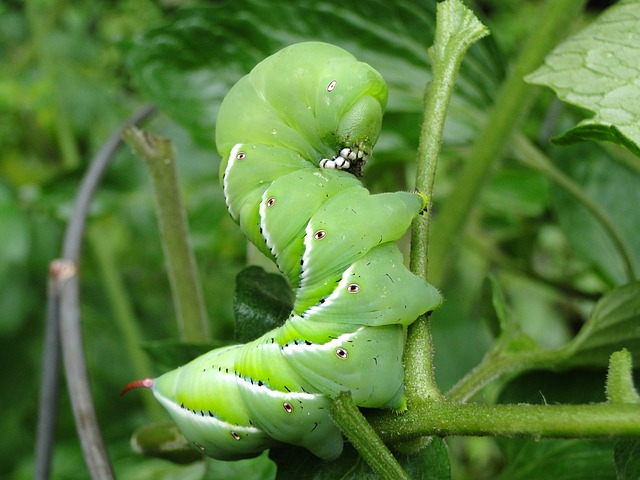
\includegraphics[scale=0.2]{ilustracje_erum/worm.jpg}
	
	\begin{itemize}
		
		\item this demand is transfered into legal regulations (see: GDPR)
		
		 $\rightarrow$ more and more institutions have to explain model predictions
		(debt collection, loans ...)
		
		\item understanding models helps improve them
	\end{itemize}
\end{frame}


\begin{frame}{Which predictions need explanation?}
	
	\begin{enumerate}
		\item Every prediction the client (or the boss) wants to understand
		
		\item Predictions that seem suspicious
	\end{enumerate}

	
	\begin{itemize}
		\item How to spot them?
	\end{itemize}
	$\rightarrow$ \textbf{model performance}
	
	$\rightarrow$ \textbf{model diagnostics}
	
	\begin{itemize}
		\item How to explain them?
	\end{itemize}
\end{frame}


\begin{frame}[fragile]{Model diagnostics: example}

		\begin{lstlisting}
library(tidyverse)
library(randomForest)
load("./rda_files/houses.rda")
hrf <- randomForest(sqm_price ~., data = houses)
head(houses)
		\end{lstlisting}
		% latex table generated in R 3.4.2 by xtable 1.8-2 package
		% Sat May 12 16:04:14 2018
		\begin{table}[ht]
			\centering
			\begin{tabular}{rrrrrrrl}
				\hline
				 rooms\_num & area & sqm\_price & year & floor & max\_floor & district \\ 
				\hline
				  3 & 89.00 & 5270 & 2007 &   2 &   2 & Krzyki \\ 
				  4 & 163.00 & 6687 & 2002 &   2 &   2 & Psie Pole \\ 
				  3 & 52.00 & 6731 & 1930 &   1 &   2 & Srodmiescie \\ 
				  4 & 95.03 & 5525 & 2016 &   1 &   2 & Krzyki \\ 
				  4 & 88.00 & 5216 & 1930 &   3 &   4 & Srodmiescie \\ 
				  2 & 50.00 & 5600 & 1915 &   3 &   4 & Krzyki \\ 
				\hline
			\end{tabular}
		\end{table}
\end{frame}

\begin{frame}[fragile]{Model diagnostics: example}
	\begin{lstlisting}
ggplot(tibble(x = houses$sqm_price, y = predict(hrf)), aes(x, y)) +
	  geom_point() +
	  geom_abline(slope = 1, intercept = 0, size = 1.2, color = "blue") +
	  theme_bw() +
	  xlab("True prices") +
	  ylab("Fitted prices")
	\end{lstlisting}
\end{frame}

\begin{frame}[fragile]{Model diagnostics: fitted vs observed}

\begin{multicols}{2}
	\includegraphics[scale=0.45]{ilustracje_erum/fitvsobs.png}

	\columnbreak
	\begin{itemize}
	\item Points on the plot should be close to the \texttt{y = x} line,
	
	\item Questions:
	
	\begin{itemize}
		
		\item is there a pattern? (For example: does the devation from true value grow as true value grows?)
		
		\item are there any points especially far from the line (meaning: points with large residuals)?
		
	\end{itemize}
	
	\item More diagnostic tools: \texttt{auditor} package
\end{itemize}
\end{multicols}
\end{frame}


\begin{frame}[fragile]{Model performance}
	\begin{lstlisting}
	library(DALEX)
rf_explainer <- explain(hrf, 
	                    data = houses, 
	                    y = houses$sqm_price)
rf_perf <- model_performance(rf_explainer)
plot(rf_perf, geom = "boxplot")
	\end{lstlisting}
\end{frame}

\begin{frame}{Model performance}
\begin{multicols}{2}
	\includegraphics[scale=0.45]{ilustracje_erum/boxres.png}
\columnbreak
	\begin{itemize}
	\item shortly summarizes the distribution of the absolute value of residuals
	\item red dot is the root mean square error
	\item we can put boxplots for several models on the same plot (simply by passing the as arguments to \texttt{plot}) to compare models
	\item boxplots help discover outliers
\end{itemize}
\end{multicols}

\end{frame}

\begin{frame}{Single prediction explanations}
	\begin{itemize}
		\item Once we identified predictions we want to explain, we need tools that will help us!
		\item Two main ideas:
		\begin{enumerate}
			\item Attribute scores to explanatory variables according to their influence on the prediction (**contributions**)
			
			\item Fit a model locally around an observation and investigate it
		\end{enumerate}
	    \item NOTE: both approaches lead to local feature importance
	\end{itemize}
\end{frame}

\begin{frame}{Single predictions explanations}
	Methods:
	\begin{enumerate}
		\item Contributions
		\begin{itemize}
			\item \texttt{breakDown} package
			\item Shapley values
		\end{itemize}
	    \item Local approximations
	    \begin{itemize}
	    	\item LIVE (Local Interpretable Visual Explanations)
	    	\item LIME (Locallly Interpretable Model-agnostic Explanations)
	    \end{itemize}
	\end{enumerate}
\end{frame}

\section{Prediction breakdown}

\begin{frame}{Break Down: general idea}
	% dodać obrazek
	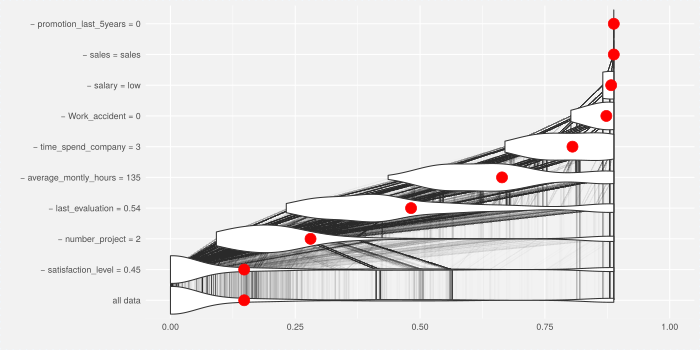
\includegraphics[scale=0.45]{ilustracje_erum/breakdown_intuition.png}
	\begin{itemize}
		\item Approach: finding \textbf{additive} feature contributions
		
		\item Contributions are assigned in a greedy manner
		
		\item Waterfall plots as a visual tool
		
		\item $\rightarrow$ intuitive interpretation
	\end{itemize}
\end{frame}

\begin{frame}[fragile]{Break Down for linear models}
	\begin{lstlisting}
linear_model <- lm(sqm_price ~., data = houses)
lm_explainer <- DALEX::explain(linear_model, 
		                       data = houses, 
		                       y = houses$sqm_price)
breakdown_linear <- single_prediction(lm_explainer, 
		                              houses[4036, -3])
plot(breakdown_linear)
	\end{lstlisting}
\end{frame}

\begin{frame}{Break Down for linear models}
	\centering
	\includegraphics[scale=0.45]{ilustracje_erum/breaklm.png}
	\begin{itemize}
		\item Contributions are scaled, so they do not depend on the scale of the data (insensitive to location/scale change)
		\item We can see actual contributions, not just the weights (as in LIME plots)
	\end{itemize}
\end{frame}


\begin{frame}[fragile]{Model-agnostic Break Down}
	\begin{lstlisting}
breakdown_explanation <- single_prediction(rf_explainer, houses[4036, -3])
plot(breakdown_explanation)
	\end{lstlisting}
\end{frame}


\begin{frame}{Model-agnostic Break Down}
	\centering
	\includegraphics[scale=0.5]{ilustracje_erum/breakma.png}
	\begin{itemize}
		\item We can see how important District and Year are in this random forest prediction
	\end{itemize}
\end{frame}

\begin{frame}[fragile]{But isn't it enough to calculate feature importance?}
	\begin{lstlisting}
global_feat_imp <- DALEX::variable_importance(rf_explainer)
plot(global_feat_imp)
	\end{lstlisting}
	\centering
	\includegraphics[scale=0.48]{ilustracje_erum/global.png}	
	
	No. Particular instances can be influenced the most by different features,
	not necessarily the ones that are most important globally.
\end{frame}

\begin{frame}{Shapley values: general idea}
  \begin{itemize}
	\item The goal is a decomposition of prediction into a \textbf{sum} of scores related to (simplified) features.
	\item The problem is solved using game theory: \textit{Shapley values}. 
	\item Variables are \textit{players} who contribute to the outcome - the prediction - and we try to \textit{pay} them accordingly to their contributions.
	\item This approach unifies several methods (including \texttt{LIME}).
  \end{itemize}
\end{frame}

\begin{frame}{Shapley values: some details}
	\begin{itemize}
		\item Exact methods exist for linear models and tree ensemble methods.
		In other cases, approximations are needed.
		
		\item The classic way: sample permutations of variables, then average contributions.
		
		\item The better way: approximation based on LIME and Shapley values for regression.
		
		\item This method has good theoretical properties, but will not produce sparse explanations
	\end{itemize}
\end{frame}

\begin{frame}[fragile]{Shapley values: example}
	\begin{lstlisting}
library(shapleyr)
library(mlr)
house_task <- makeRegrTask(data = houses, target = "sqm_price")
house_rf_mlr <- train("regr.randomForest", house_task)	

shapley_explanation <- shapley(4036,
                               task = house_task,
                               model = house_rf_mlr)
class(shapley_explanation) <- c("shapley.singleValue", "list")
plot(shapley_explanation)
	\end{lstlisting}
\end{frame}

\begin{frame}[fragile]{Shapley values: example}
	\centering
	\includegraphics[height = 120px, width = 300px]{ilustracje_erum/shapley.png}
	\begin{itemize}
		\item \textbf{0} is the mean of all predictions
		
		\item the \textbf{black dot} is the prediction we are explaining
		
		\item values and the plot describe how we move from the global mean of predictions to this particular predictions
		
		\item most important features are the ones that help move the most
		
		\item many different \textit{paths} from the mean to the predictions are considered and averaged
	\end{itemize}
\end{frame}

\begin{frame}[fragile]{Shapley values: example}
\begin{lstlisting}
gather(shapley_explanation$values, "feature", "shapley.score")
\end{lstlisting}
% latex table generated in R 3.4.2 by xtable 1.8-2 package
% Sat May 12 16:46:58 2018
\begin{table}[ht]
	\centering
	\begin{tabular}{rll}
		\hline
		& feature & shapley.score \\ 
		\hline
		1 & \_Id & 4036 \\ 
		2 & \_Class &  \\ 
		3 & rooms\_num & -32.25 \\ 
		4 & area & -597.239 \\ 
		5 & year & 461.175 \\ 
		6 & floor & -137.767 \\ 
		7 & max\_floor & -32.202 \\ 
		8 & district & -122.961 \\ 
		\hline
	\end{tabular}
\end{table}
\end{frame}



\begin{frame}{Time to practice!}
	
\end{frame}


\begin{frame}[fragile]{Exercises}
1. Run the following code to fit random forest, linear regression and SVM to the housing prices data.
\begin{lstlisting}
library(tidyverse)
library(live)
library(DALEX)
library(randomForest)
library(e1071)
library(auditor)
load("./rda_files/houses.rda")

set.seed(33)
house_rf <- randomForest(sqm_price ~., data = houses)
house_svm <- svm(sqm_price ~., data = houses)
house_lm <- lm(sqm_price ~., data = houses)
\end{lstlisting}
Create DALEX explainer object for each of the models. 
Create and compare boxplots of residuals for all the models (\texttt{model\_performance}). 
\end{frame}

\begin{frame}{Exercises}
\begin{itemize}
	\item Which model is the best?
	\item Are there any outlying predictions?
	\item Find the observation with the largest absolute value of residual among houses cheaper than 7000 PLN. 
\end{itemize}

TIP: object returned by \texttt{model\_performance} function is a data frame with colnames 
\textit{predicted}, \textit{observed}, \textit{diff} and \textit{label}.
\end{frame}

\begin{frame}[fragile]{Exercises}
2. Create single prediction explainers for the instance chosen in Exercise 1.
Create Break Down plots for each of the observations. What are the keys factors that drive the prediction?
Are they the same for every model?

3. Run the following code to train model random forest model using \textit{mlr} interface 
(this is necessary for `shapleyR` package).

\begin{lstlisting}
library(mlr)
load("./rda_files/houses.rda")
n_obs <- 1189

house_task <- makeRegrTask(data = houses, target = "sqm_price")
house_rf_mlr <- train("regr.randomForest", house_task)
\end{lstlisting}
Use shapleyR package to calculate Shapley values for prediction chosen in Exercise 1 (its index is in \texttt{n\_obs} object). 
Are the results consistent with Break Down results from Exercise 2?
Draw a plot of Shapley values.

TIP: remember to set class of the object returned by \texttt{shapley} function to \texttt{shapley.singleValue} before using \texttt{plot}.

\end{frame}

\begin{frame}{Bonus exercises}
	\begin{itemize}
		\item Draw plots of fitted vs observed values for each of these models. Can you spot any problems with the predictions? Are the prices usually underestimated of overestimated?
		\item Create variable importance explainer. Compare global variable importance to scores obtained in Exercise 2 and Exercise 3.
	\end{itemize}	
	
\end{frame}

\section{Local approximations}

\begin{frame}{LIME: General idea}
	\begin{center}
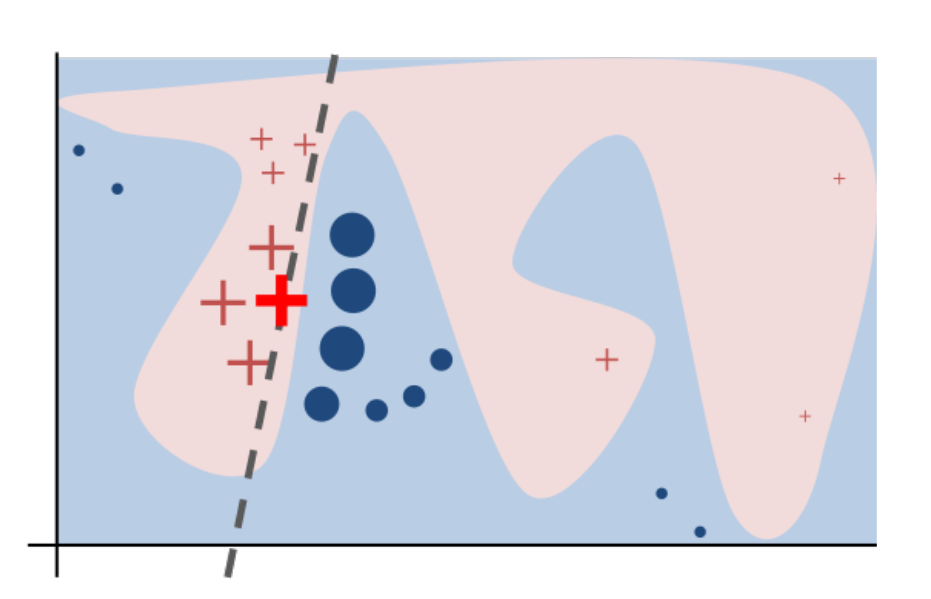
\includegraphics[scale=0.4]{ilustracje_erum/lime_intuition.png}		
	\end{center}
\end{frame}

\begin{frame}{LIME: some details}
	\begin{itemize}
\item Observations are transformed to \textit{interpretable input space}

\item Gaussian sampling for tabular, uniform sampling from interpretable inputs for image/text.

\item Scores for new observation are weighted by the distance from original observation.

\item Variable selection is usually based on ridge/lasso regression.

\item Weights are assigned to interpretable inputs to decide if they \textit{vote} for or against a given label.

\item Note: method depends on many hyperparameters
	\end{itemize}
\end{frame}

\begin{frame}[fragile]{LIME: example}
\begin{lstlisting}
library(lime)

explained_prediction <- houses[4036, ]

lime_explainer <- lime(houses,
                  model = house_rf_mlr)
lime_explanation <- lime::explain(houses[4036, ],
                                  explainer = lime_explainer,
                                  n_features = 5)
plot_features(lime_explanation)	
\end{lstlisting}
\end{frame}

\begin{frame}{LIME: example}
	\centering
\includegraphics[scale = 0.53]{ilustracje_erum/lime.png}
\begin{itemize}
	\item weights from ridge regression are on the plot (NOT weights multiplied by actual feature values)
	\item positive weights are \textit{votes for}, negative weights are \textit{against}
\end{itemize}
\end{frame}

\begin{frame}{LIVE: general idea}
   \begin{itemize}
   	\item Modification of \texttt{LIME} for tabular data and regression problems with emphasis on model visualization.
   	\item Similar observations for \textit{fake} dataset are sampled from empirical distributions.
    \item Variable selection is possible (LASSO, then explanation model is fitted to selected features).
   \end{itemize}
\end{frame}

\begin{frame}{LIVE: some details}
	\begin{itemize}
	\item Two methods of creating the new dataset are available: by permuting each variable and by changing one feature per observations (method does matter)
	\item We can control which variables are allowed to vary through \texttt{fixed\_variables} variable argument to \texttt{sample\_locally} (keeping date/factor/correlated variables unchanged)
	\item features can be standardized before fitting explanation model
	\item Black box model can be pre-trained or it can be trained using \texttt{mlr} interface
	\item Hyperparameters of both black box and explanation models can be set
	\end{itemize}
	
\end{frame}

\begin{frame}[fragile]{LIVE: example}
\begin{lstlisting}
library(live)
library(mlr)

new_dataset <- sample_locally2(data = houses,
                               explained_instance = houses[4036, ],
                               explained_var = "sqm_price",
                               size = 1000)
with_predictions <- add_predictions2(new_dataset, hrf)
live_explanation <- fit_explanation2(with_predictions, 
                                     "regr.lm", 
                                     standardize = TRUE)
\end{lstlisting}
\end{frame}

\begin{frame}[fragile]{LIVE: example}
\begin{lstlisting}
live_explanation

Dataset: 
  Observations:  500 
  Variables:  7 
  Response variable:  sqm_price 
Explanation model: 
  Name: regr.lm 
  Variable selection wasnt performed 
  Weights present in the explanation model 
  R-squared: 0.8923
\end{lstlisting}
\begin{itemize}
	\item Default method of sampling is \texttt{live}
	\item Default explanation model is linear regression and distance is measured (weights are assigned) by gaussian kernel
\end{itemize}
\end{frame}

\begin{frame}[fragile]{Plot local model structure: forest plot}
	\begin{center}
	\includegraphics[scale=0.6]{ilustracje_erum/forest.png}		
	\end{center}
\end{frame}

\begin{frame}[fragile]{Plot local variable contributions: waterfall plot}
	\begin{center}
		\includegraphics[scale=0.6]{ilustracje_erum/waterfall.png}
	\end{center}
\end{frame}

\begin{frame}{Acknowledgement}
	\centering
	\includegraphics[scale=0.5]{ilustracje_erum/uwr.png}
\end{frame} 


\begin{frame}{Time to practice!}
  
\end{frame}


\begin{frame}[fragile]{Exercises}
4. Simulate new data around the observation from Exercise 1 (row 1189) and the add random forest predictions (from \texttt{house\_rf} object). Then fit a linear model locally.
	
TIP: remember to load \texttt{mlr} package.
TIP2: don't use too small \texttt{size} for the simulated dataset. I recommend at least 1000.
	
5. Visualize approximation created in Exercise 4.
Use \texttt{plot\_explanation2} function to create a forest plot of the linear model and then the Break Down plot. 

6. Use \texttt{lime} package to approximate random forest model around prediction chosen in  Exercise 1.
Follow the \texttt{lime} work flow: create an explainer, approximate the model around the explained instance and then use \texttt{plot\_features} function to see, how features influence this prediction.

TIP: use \texttt{house\_rf\_mlr} object from Exercise 3, because \texttt{lime} works well with \texttt{mlr} objects.

\end{frame}

\begin{frame}[fragile]{Bonus exercises}

1. Use \texttt{add\_predictions} function to add SVM and LM predictions to the simulated dataset. Compare plots for all three models.
	
2. Run the following code to see largest residuals for \textit{Psie Pole} district.
\begin{lstlisting}
library(tidyverse)
  houses %>%
  mutate(id = 1:n()) %>%
  mutate(rf_pred = predict(house_rf)) %>%
  mutate(abs_res = abs(sqm_price - rf_pred)) %>%
  arrange(desc(abs_res)) %>%
  filter(sqm_price < 7000,
         district == "Psie Pole") %>%
  head(5)

n_obs2 <- 5830
\end{lstlisting}
Using \texttt{live} package, fit a linear model around the top observation.
Compare waterfall plots for this prediction and the prediction from Exercise 5.
How are they different?

\end{frame}

%	\begin{frame}[allowframebreaks]{References}
%		\nocite{*}
%		\bibliographystyle{amsalpha}
%		\bibliography{berlin.bib}
%	\end{frame}
	
\end{document}
